\documentclass[a4paper]{article}

\usepackage{fullpage} % Package to use full page
\usepackage{parskip} % Package to tweak paragraph skipping
\usepackage{amsmath}
\usepackage{hyperref}

\usepackage{pgfplots}


\usepackage{tikz} % Package for drawing
    \usetikzlibrary{positioning}

\tikzset{basic/.style={draw,fill=blue!20,text width=1em,text badly centered}}
\tikzset{input/.style={basic,circle}}
\tikzset{weights/.style={basic,rectangle,text width = }}
\tikzset{functions/.style={basic,circle,fill=blue!10}}


\title{NN-Homework}
\author{Pengfei (Leonard) Li}
%\date{1982-06-19}

\begin{document}

\maketitle

\section{Problem 1}
\begin{tikzpicture}
\begin{axis}[
    axis lines=middle,
    xmin=-1, xmax=2,
    ymin=-1, ymax=2,
    xtick=\empty, ytick=\empty,
    xlabel={A}, ylabel={B}
]
\addplot [only marks] table {
1 1
};
\addplot [only marks, mark=o] table {
0 0
0 1
1 0
};
\addplot [domain=-1:2, samples=2, dashed] {-1*x+1.5};
\end{axis}
\end{tikzpicture}

This is the decision surface of A AND B, where solid circles refers to TRUE, and empty ones FLASE. Its output is given by
$$o(A, B) = sgn(w_0 + w_1*A + w_2*B) $$
The weights $\vec{w}$ satisfies the following system  of in-equations. 
$$\begin{cases} w_0+w_2<0 \\  w_0+w_1<0 \\  w_0+w_1+w_2>0 \end{cases}$$

A perceptron with possible weights is
\begin{center}
 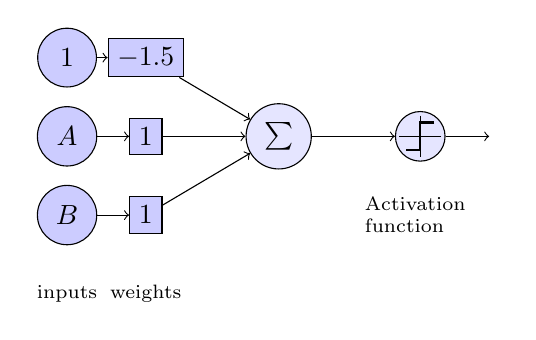
\begin{tikzpicture}
        \node[functions] (center) {};
        \node[below of=center,font=\scriptsize,text width=4em] {Activation function};
        \draw[thick] (0.5em,0.5em) -- (0,0.5em) -- (0,-0.5em) -- (-0.5em,-0.5em);
        \draw (0em,0.75em) -- (0em,-0.75em);
        \draw (0.75em,0em) -- (-0.75em,0em);
        \node[right of=center] (right) {};
            \path[draw,->] (center) -- (right);
        \node[functions,left=3em of center] (left) {$\sum$};
            \path[draw,->] (left) -- (center);
        \node[weights,left=3em of left] (1) {$1$} -- (1) node[input,left of=1] (l1) {$A$};
            \path[draw,->] (l1) -- (1);
            \path[draw,->] (1) -- (left);
        \node[weights,below of=1] (2) {$1$} -- (2) node[input,left of=2] (l2) {$B$};
            \path[draw,->] (l2) -- (2);
            \path[draw,->] (2) -- (left);
        \node[weights,above of=1] (0) {$-1.5$} -- (0) node[input,left of=0] (l0) {$1$};
            \path[draw,->] (l0) -- (0);
            \path[draw,->] (0) -- (left);
        \node[below of=l2,font=\scriptsize] {inputs};
        \node[below of=2,font=\scriptsize] {weights};
    \end{tikzpicture}
\end{center}



\section{Problem 2}
\begin{tikzpicture}
\begin{axis}[
    axis lines=middle,
    xmin=-1, xmax=2,
    ymin=-1, ymax=2,
    xtick=\empty, ytick=\empty,
    xlabel={A}, ylabel={B}
]
\addplot [only marks] table {
1 1
0 1
1 0
};
\addplot [only marks, mark=o] table {
0 0
};
\addplot [domain=-1:2, samples=2, dashed] {-1*x+0.5};
\end{axis}
\end{tikzpicture}

This is the decision surface of A OR B, where solid circles refers to TRUE, and empty ones FLASE. Its output is given by
$$o(A, B) = sgn(w_0 + w_1*A + w_2*B) $$
The weights $\vec{w}$ satisfies the following system  of in-equations. 
$$\begin{cases} w_0+w_2>0 \\  w_0+w_1>0 \\  w_0<0 \end{cases}$$

A perceptron with possible weights is
\begin{center}
 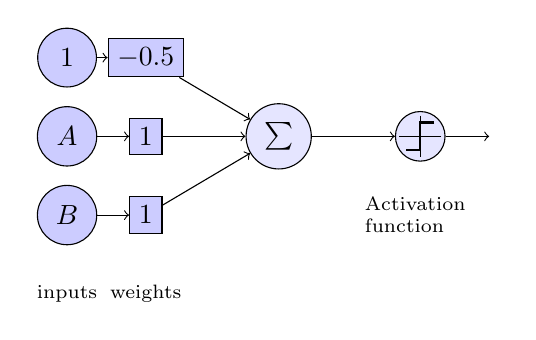
\begin{tikzpicture}
        \node[functions] (center) {};
        \node[below of=center,font=\scriptsize,text width=4em] {Activation function};
        \draw[thick] (0.5em,0.5em) -- (0,0.5em) -- (0,-0.5em) -- (-0.5em,-0.5em);
        \draw (0em,0.75em) -- (0em,-0.75em);
        \draw (0.75em,0em) -- (-0.75em,0em);
        \node[right of=center] (right) {};
            \path[draw,->] (center) -- (right);
        \node[functions,left=3em of center] (left) {$\sum$};
            \path[draw,->] (left) -- (center);
        \node[weights,left=3em of left] (1) {$1$} -- (1) node[input,left of=1] (l1) {$A$};
            \path[draw,->] (l1) -- (1);
            \path[draw,->] (1) -- (left);
        \node[weights,below of=1] (2) {$1$} -- (2) node[input,left of=2] (l2) {$B$};
            \path[draw,->] (l2) -- (2);
            \path[draw,->] (2) -- (left);
        \node[weights,above of=1] (0) {$-0.5$} -- (0) node[input,left of=0] (l0) {$1$};
            \path[draw,->] (l0) -- (0);
            \path[draw,->] (0) -- (left);
        \node[below of=l2,font=\scriptsize] {inputs};
        \node[below of=2,font=\scriptsize] {weights};
    \end{tikzpicture}
\end{center}




\section{Problem 3}
\begin{tikzpicture}
\begin{axis}[
    axis lines=middle,
    xmin=-1, xmax=2,
    ymin=-1, ymax=2,
    xtick=\empty, ytick=\empty,
    xlabel={A}, ylabel={B}
]
\addplot [only marks] table {
0 1
1 0
};
\addplot [only marks, mark=o] table {
0 0
1 1
};
\end{axis}
\end{tikzpicture}

There is no possible decision surface that could separate empty and solid circles, as we suppose A and B are different. 
But if A and B are the same 














\section{Exploring the derivative using Sage}

The definition of the limit of $f(x)$ at $x=a$ denoted as $f'(a)$ is:

\begin{equation}
f'(a) = \lim_{h\to0}\frac{f(a+h)-f(a)}{h}
\end{equation}

The following code can be used in sage to give the above limit:

\begin{verbatim}
def illustrate(f, a):
    """
    Function to take a function and illustrate the limiting definition of a derivative at a given point.
    """
    lst = []
    for h in srange(.01, 3, .01):
    	lst.append([h,(f(a+h)-f(a))/h])
    return list_plot(lst, axes_labels=['$x$','$\\frac{f(%.02f+h)-f(%.02f)}{h}$' % (a,a)])
\end{verbatim}



If we want to plot the tangent at a point $\alpha$ to a function we can use the following:

\begin{align}
y=&ax+b&&\text{(definition of a straight line)}\nonumber\\
  &f'(a)x+b&&\text{(definition of the derivative)}\nonumber\\
  &f'(a)x+f(a)-f'(a)a&&\text{(we know that the line intersects $f$ at $(a,f(a))$}\nonumber
\end{align}

We can combine this with the approach of the previous piece of code to see how the tangential line converges as the limiting definition of the derivative converges:

\begin{verbatim}
def convergetangentialline(f, a, x1, x2, nbrofplots=50, epsilon=.1):
    """
    Function to make a tangential line converge
    """
    clrs = rainbow(nbrofplots)
    k = 0
    h = epsilon
    p = plot(f, x, x1, x2)
    while k < nbrofplots:
        tangent(x) = fdash(f, a, h) * x + f(a) - fdash(f, a, h) * a
        p += plot(tangent(x), x, x1, x2, color=clrs[k])
        h += epsilon
        k += 1
    return p
\end{verbatim}

The plot shown in Figure \ref{lines} shows how the lines shown converge to the actual tangent to $1-x^2$ as $x=2$ (the red line is the `closest' curve).

%\begin{figure}[!htbp]
%\begin{center}
%\includegraphics[width=8cm]{sage0.png}
%\end{center}
%\caption{Lines converging to the tangent curve as $h\to0$.}\label{lines}
%\end{figure}

Note here that the last plot is given using the \textbf{real} definition of the derivative and not the approximation.

\section{Conclusions}

In this report I have explored the limiting definition of the limit showing how as $h\to 0$ we can visualise the derivative of a function. The code involved \url{https://sage.maths.cf.ac.uk/home/pub/18/} uses the differentiation capabilities of Sage but also the plotting abilities.

There are various other aspects that could be explored such as symbolic differentiation rules. For example:

$$\frac{dx^n}{dx}=(n+1)x^{n}\text{ if }x\ne-1$$

Furthermore it is interesting to not that there exists some functions that \textbf{are not} differentiable at a point such as the function $f(x)=\sin(1/x)$ which is not differentiable at $x=0$. A plot of this function is shown in Figure \ref{notdiff}.




\end{document}